\subsection{Вибрационные гироскопы}

Вибрационные гироскопы представляют собой класс инерциальных датчиков, в которых для измерения угловой скорости используется не вращение постоянного ротора, а колебательное движение (вибрация) чувствительного элемента \cite{mems_sensors}. Их развитие, особенно в области микроэлектромеханических систем (МЭМС), совершило революцию, сделав гироскопические технологии массовыми и доступными.

Для корректного анализа работы вибрационных гироскопов, в частности МЭМС-датчиков угловой скорости, необходимо строгое рассмотрение кинематики движения в неинерциальных системах отсчёта, задаваемое теоремой Кориолиса \cite{persson2005coriolis}.

% -----------------------------------------------------------------------------

\subsubsection{Теорема Кориолиса}

Рассмотрим движение материальной точки в двух системах координат: инерциальной системе OXYZ и неинерциальной системе Ox'y'z', которая вращается относительно инерциальной с мгновенной угловой скоростью $\vec{\omega}$.

Тогда абсолютная скорость рассматриваемой материальной точки будет по теореме сложения скоростей будет равна:

\begin{equation}
	\vec{v} = \vec{v_{0}} + [\vec{\omega}, \vec{R}] + \vec{v_{r}}
\end{equation}

где $\vec{R}$ - радиус-вектор точки относительно мгновенного центра скоростей 
O, $\vec{V_{0}}$ - переносная скорость точки, $\vec{V_{r}}$ - её относительная скорость.

Продифференцируем это равенство по времени:

\begin{equation}
	\frac{d}{dt} \vec{v} = \frac{d}{dt} \vec{v}_0 + \frac{d}{dt} \left[ \vec{\omega} \times \vec{R} \right] + \frac{d}{dt} \vec{v}_r.
\end{equation}


Найдём значение каждого слагаемого в инерциальной системе координат:

\[
\frac{d}{dt} \vec{v}_0 = {\vec{a}}_0,
\]

\[
\frac{d}{dt} \left[ \vec{\omega} \times \vec{R} \right] = \left[ \vec{\varepsilon} \times \vec{R} \right] + \left[ \vec{\omega} \times \frac{d}{dt} \vec{R} \right] = \left[ \vec{\varepsilon} \times \vec{R} \right] + \left[ \vec{\omega} \times \left[ \vec{\omega} \times \vec{R} \right] \right] + \left[ \vec{\omega} \times \vec{v}_r \right],
\]

\[
\frac{d}{dt} \vec{v}_r = \left[ \vec{\omega} \times \vec{v}_r \right] + \frac{d_r \vec{v}_r}{dt},
\]

где \(\vec{a}_r\) — линейное ускорение точки относительно системы \(Ox'y'z'\), \(\vec{\varepsilon} = \frac{d\vec{\omega}}{dt}\) — угловое ускорение системы \(Ox'y'z'\).

Таким образом, имеем:

\[
\frac{d}{dt} \vec{v} = \ddot{\vec{a}}_0 + \left[ \vec{\varepsilon} \times \vec{R} \right] + \left[ \vec{\omega} \times \left[ \vec{\omega} \times \vec{R} \right] \right] + \ddot{\vec{a}}_r + 2 \left[ \vec{\omega} \times \vec{v}_r \right].
\]

\hspace{1cm}

Полученное равенство служит математическим выражением теоремы Кориолиса: Абсолютное ускорение точки в сложном движении равно геометрической сумме её переносного ускорения, относительного ускорения и добавочного кориолисова ускорения, равного \(2 \left[ \vec{\omega} \times \vec{v}_r \right]\).


При переходе к уравнению движения во вращающейся системе отсчёта это ускорение, взятое с обратным знаком и умноженное на массу точки, интерпретируется как сила инерции Кориолиса:

\begin{equation}
	F_{c} = -m · a_{c} = -2m [\vec{\omega}, \vec{v_{r}}].
\end{equation}

\vspace{0.5cm}

\begin{figure}[ht]
	\centering
	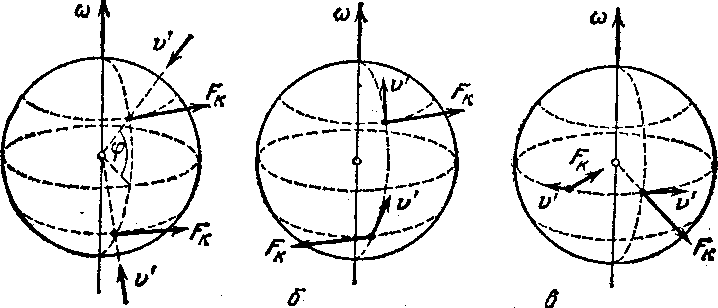
\includegraphics[width=0.7\textwidth]{images/theory/гироскопы/иллюстрация силы Кориолиса.png}
	\caption{Иллюстрация силы Кориолиса}
\end{figure}

В контексте вибрационных гироскопов $v_{r}$ — это скорость контролируемого колебательного движения чувствительной массы (режим привода), а $\omega$ — измеряемая угловая скорость корпуса прибора. Возникающая при этом сила Кориолиса $F_{c}$ вызывает вторичные колебания массы в перпендикулярном направлении (режим считывания), амплитуда которых пропорциональна $\omega$. Следовательно, теорема Кориолиса предоставляет фундаментальную физико-математическую основу для преобразования измеряемого вращения в измеримое механическое перемещение, что является ключевым принципом действия всего класса вибрационных гироскопических датчиков.

% -----------------------------------------------------------------------------

\subsubsection{Одноосевой МЕМС-гироскоп с вибрирующим кремниевым кольцом}

Описываемые гироскопы относятся к классу вибрационных твердотельных датчиков и характеризуются отсутствием классических вращающихся масс или подшипников. Единственным подвижным элементом является упругое сенсорное кольцо из монокристаллического кремния, совершающее микроскопические колебания, что обеспечивает исключительную долговечность и стойкость к механическим нагрузкам.

Принцип действия основан на измерении вызванной силой Кориолиса прецессии стоячей волны в резонаторе, что позволяет определять величину и направление приложенной угловой скорости \cite{mems_sensors}.

Ключевые элементы конструкции и режимы работы:

\begin{itemize}
	\item Чувствительный элемент: Кольцевой резонатор, подвешенный на упругих спицах или непосредственно на центральном основании.
	\item Система возбуждения и контроля первичной моды: По периметру кольца симметрично расположены восемь преобразователей. Одна пара выполняет роль приводов первичного движения, другая — первичных считывающих преобразователей. Они расположены на главных ортогональных осях, образуя замкнутую систему автоматического регулирования с ASIC-контроллером. Эта система возбуждает и поддерживает стабильные резонансные колебания первичной моды с частотой около 22 кГц. В этом состоянии кольцо деформируется, принимая квазиэллиптическую форму.
	\item Система считывания вторичной моды: Две дополнительные пары вторичных считывающих преобразователей расположены по осям, смещенным на 45° относительно главных. При отсутствии вращения радиальное движение в этих точках отсутствует.
\end{itemize}


\begin{figure}[ht]
	\centering
	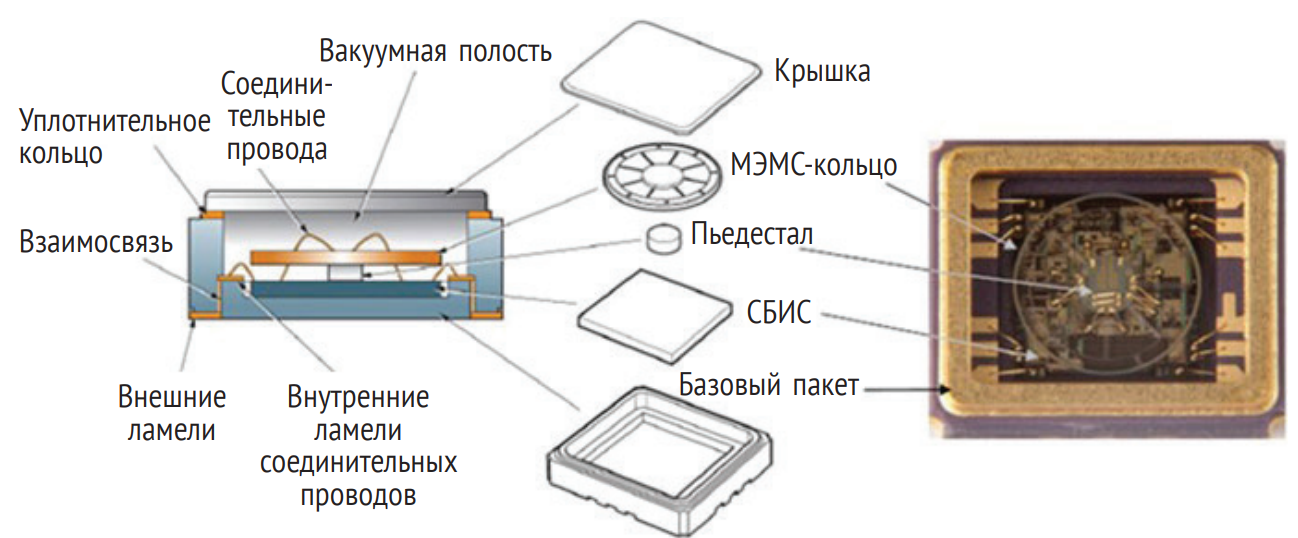
\includegraphics[width=0.9\textwidth]{images/theory/гироскопы/основные детали кремниевого гироскопа.png}
	\caption{Основные детали кремниевого гироскопа}
\end{figure}


\subsubsection{Принцип измерения угловой скорости}

Когда гироскоп начинает вращаться с угловой скоростью $\Omega$, на колеблющиеся участки кольца действуют силы Кориолиса. Эти силы, распределенные по периметру, не совпадают по фазе с первичными колебаниями и вызывают возбуждение вторичной (квадратурной) моды колебаний. Это приводит к прецессии узловой картины стоячей волны вокруг оси кольца. В результате на электродах вторичного считывания возникает сигнал радиального смещения, строго пропорциональный приложенной угловой скорости \cite{mems_sensors}.



\begin{figure}[H]
	\centering
	\begin{subfigure}{0.48\textwidth}
		\centering
		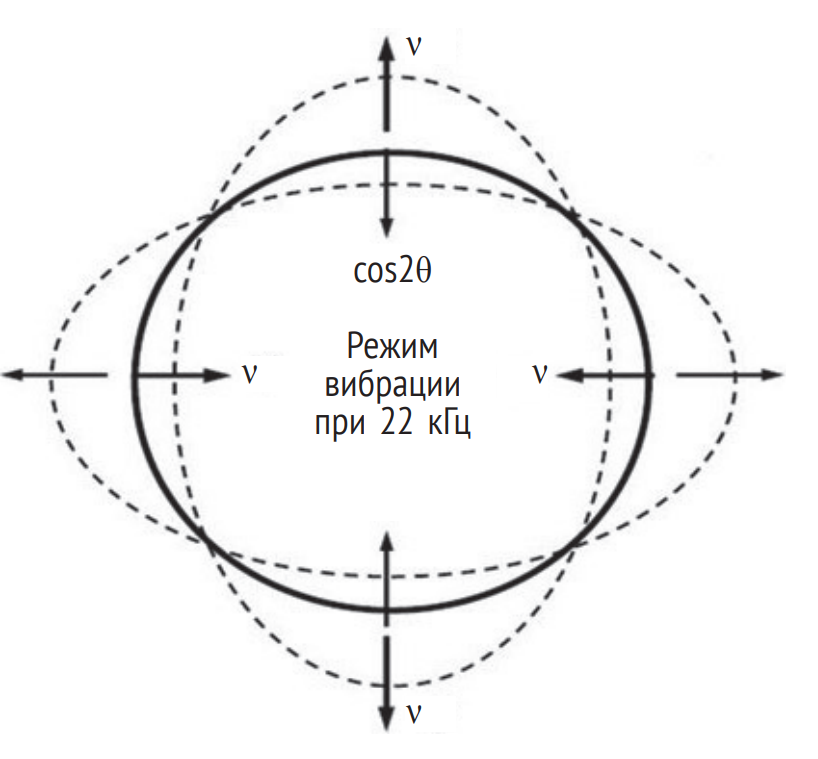
\includegraphics[width=0.7\textwidth]{images/theory/гироскопы/иллюстрация кольца в покое.png}
		\caption{Иллюстрация кольца \\ в состоянии покоя}
	\end{subfigure}
	\hfill
	\begin{subfigure}{0.48\textwidth}
		\centering
		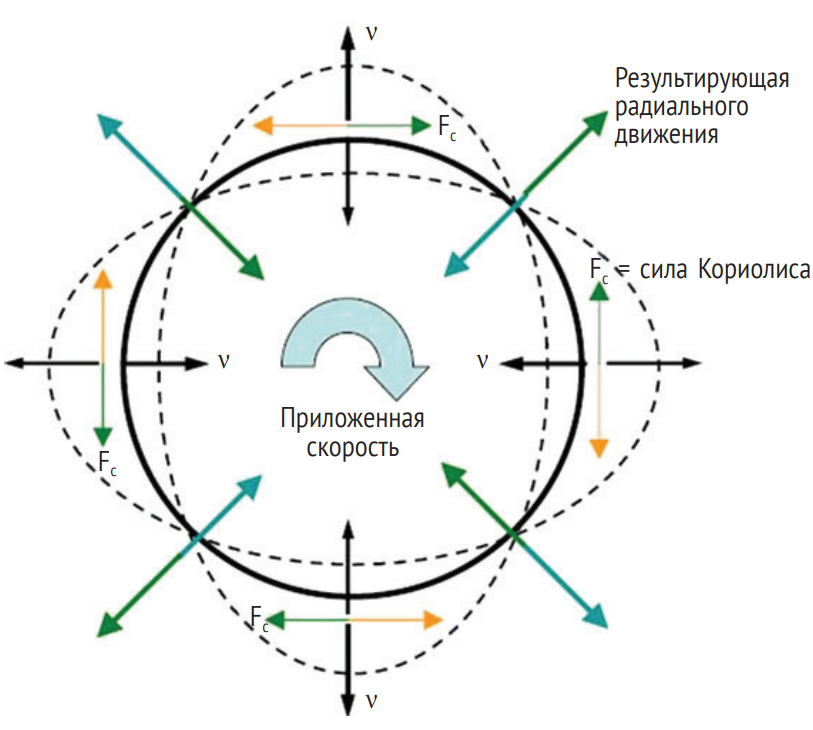
\includegraphics[width=0.7\textwidth]{images/theory/гироскопы/состояние гироскопа без движения.png}
		\caption{Иллюстрация состояния включенного гироскопа в отсутствие движения}
	\end{subfigure}
	\caption{Иллюстрации состояний вибрирующего кольца}
\end{figure}








